\documentclass[a4paper, 12pt]{article}

\usepackage[utf8]{inputenc}
\usepackage[russian]{babel}
\usepackage{icomma} % smart comma(spaces could be in formulas)
\usepackage{amsmath,amsfonts,amssymb,amsthm,mathtools} %AMS

\title{\centering Отчет по заданию №1 "\textbf{Метрические алгоритмы классификации}". Алгоритм k ближайших соседей}
\date{\vspace*{\fill}Кузьмин Никита, \\ cтудент 3 курса факультета ВМК \\ кафедры ММП, \\ МГУ \\ 2019, \\ Октябрь}

% Свои команды и функции
\DeclareMathOperator{\sgn}{\mathop{sgn}}

%Убирает все номера формул, на которые не ссылок в тексте:
%\mathtoolsset{showonlyrefs=true}

\usepackage{extsizes} % Возможность сделать 14 шрифт в documentclass при article
\usepackage{geometry} % Просто способ задавать поля
    \geometry{top=25mm}
    \geometry{bottom=35mm}
    \geometry{left=35mm}
    \geometry{right=20mm}
   
\usepackage{fancyhdr} % Колонтитулы
    \pagestyle{fancy}
    \renewcommand{\headrulewidth}{0pt} % Толщина линейки, отчеркивающей верхний колонтитул
%    \lfoot{Нижний левый}
%    \rfoot{Нижний правый}
%    \rhead{Верхний правый}
%    \chead{Верхний в центре}
%    \lhead{Верхний левый}

\usepackage{setspace} % Интерлиньяж
%\onehalfspacing
%\doublespacing
%\singlespacing

\usepackage{hyperref}  % Гиперссылки
\usepackage[usernames,dvipsnames,svgnames,table,rgb]{xcolor}
\hypersetup{
    unicode=true,
    pdftitle={cheat_sheet}, % Заголовок
    pdfauthor={Кузьмин Никита, ММП 317},
    pdfcreator={Кузьмин Никита, ММП 317},
    colorlinks=true, % false - ссылки в рамках; true - цветные ссылки
    linkcolor=red,   % внутренние ссылки
    citecolor=green, % на библиографию
    filecolor=magenta, % на файлы
    urlcolor=blue % на URL
}

%\renewcommand{\familydefault}{\sfdefault} % Убирает засечки у шрифта

%\usepackage{multicol} % Позволяет писать текст в несколько колонок



\begin{document}
\maketitle

\section{Свой титульный лист}
\newpage
\thispagestyle{empty}
\begin{center}
    \textit{Московский Государственный Университет имени М. В. Ломоносова\\
        Факультет выислительной математики и кибернетики}
    \vspace{0.5ex}
    \vspace{30ex}
    
    Отчет по заданию №1 "\textbf{Метрические алгоритмы классификации}". Алгоритм k ближайших соседей
    
\end{center}
\vspace{13ex}
\begin{flushright}
    \noindent % Убирает красную строку
    \vfill
    \textit{Кузьмин Н. В.}
    \\
    \textit{студент кафедры ММП \\ 317 группа}
    
\end{flushright}
\begin{center}
    Октябрь,
    
    2019
\end{center}

\newpage
\section{Первый раздел}\label{razdel}
\subsection{Subsection}\label{podrazdel}
В разделе \ref{razdel} начинается документ
Подраздел \ref{podrazdel}  

\newpage
Первый абзац
$ 2 + 2 = 4$
\[2 + 3 = 5\]
$2,4$

$(2, 4)$
\begin{equation}\label{eq:mrmc}
MR=MC
\end{equation}

\eqref{eq:mrmc} на стр \pageref{eq:mrmc} ---  условие максимизации прибыли

\[\frac{1+\dfrac{4}{2}}{6} = 0,5\]

\subsection{Скобки}
плохой размер скобок:
\[(2 + \frac{9}{3})\times 5 = 25\]
хороший размер скобок:
\[\left(2 + \frac{9}{3}\right)\times 5 = 25\]

\[[2+3]\]
Обязательно ставить \ перед фигурными скобками, иначе они не отобразятся!
\[\{2+3\}\]

\subsection{Стандартные функции}

$\sin x = 5$, 
$\ln x = 5$,
$\sgn x = 1$

\subsection{Символы}\label{symbols}

$2\times 2 \ne 5$

$A \cap B,A \cup B$

\subsection{Диакритические знаки}

$\bar x =5$, $\tilde{x} = 8$

Если хотим отрицание над несколькими переменными:
\[\bar{xyz} = 1\]

Но так вышло плохо, исправим:
\[\overline{xyz} = 1\]

\[\widetilde{xywew} = 5\]

\subsection{Буквы других алфавитов}

\[tg(\alpha) = 1\]
Для больших греческих букв:
\[tg(\Phi) = 5\]
Некоторые правила написания греческих букв.
\[\epsilon\]
Эпсилон выглядит не очень привычно, изменим:
\[\varepsilon\]

\section{Формулы в несколько строк}

\subsection{Очень длинные формулы}
\begin{multline}
1+2+3+4+5+6+7 \dots + \\ + 50 + 51 + 52 + 53 + 53 + 54 + 55+ 56 + 57 + \dots + \\ + 96 + 97 + 98 + 99 + 100
\end{multline}

Несколько формулы, их выравнивание с помощью align. Нечетные \& отвечают за выравнивание внутри столбца, а четные \& за создание нового столбца
\begin{align}
2\times 2 &= 4& 6\times 8 &= 48\\
3\times 3 &= 9& a + b &= c\\
10\times 10 &= 100& \frac{1}{5} &= 0.2
\end{align}

Если не хотим нумеровать - align*:
\begin{align*}
2\times 2 &= 4& 6\times 8 &= 48\\
3\times 3 &= 9& a + b &= c\\
10\times 10 &= 100& \frac{1}{5} &= 0.2
\end{align*}

Для нумерации группы формул:
\begin{equation}
\begin{aligned}
2\times 2 &= 4& 6\times 8 &= 48\\
3\times 3 &= 9& a + b &= c\\
10\times 10 &= 100& \frac{1}{5} &= 0.2
\end{aligned}
\end{equation}


\subsection{Системы уравнений}
Обычная:
\[\left\{
\begin{aligned}
2\times 2 &= 4& 6\times 8 &= 48\\
3\times 3 &= 9& a + b &= c\\
10\times 10 &= 100& \frac{1}{5} &= 0.2
\end{aligned}\right.
\]
С условиями:
\[
|x| = \begin{cases}
x, &\text{if } x \ge 0 \\
-x, &\text{if } x < 0
\end{cases}
\]

\section{Матрицы}
Матрица в круглых скобках:
\[
\begin{pmatrix}
a_{11} & a_{12} & a_{13}\\
a_{21} & a_{22} & a_{23}\\
a_{31} & a_{32} & a_{33}\\
\end{pmatrix}
\]
Определитель матрицы:
\[
\begin{vmatrix}
a_{11} & a_{12} & a_{13}\\
a_{21} & a_{22} & a_{23}\\
a_{31} & a_{32} & a_{33}\\
\end{vmatrix}
\]
Матрица в квадратных скобках(используем tag для своей нумерации)
\[
\begin{bmatrix}
a_{11} & a_{12} & a_{13}\\
a_{21} & a_{22} & a_{23}\\
a_{31} & a_{32} & a_{33}\\
\end{bmatrix}\tag{MATRIX}
\]

\section{Кегль}
    \begin{table}[h!]
        \caption{Размеры шрифта}
        \centering
        \begin{tabular}{|c|c|}
            \hline	\verb|\tiny|      & \tiny        крошечный \\
            \hline	\verb|\scriptsize|   & \scriptsize  очень маленький\\
            \hline \verb|\footnotesize| & \footnotesize  довольно маленький \\
            \hline \verb|\small|        &  \small        маленький \\
            \hline \verb|\normalsize|   &  \normalsize  нормальный \\
            \hline \verb|\large|        &  \large       большой \\
            \hline \verb|\Large|        &  \Large       еще больше \\[5pt]
            \hline \verb|\LARGE|        &  \LARGE       очень большой \\[5pt]
            \hline \verb|\huge|         &  \huge        огромный \\[5pt]
            \hline \verb|\Huge|         &  \Huge        громадный \\ \hline
        \end{tabular}
    \end{table}

Какой-\scriptsize нибудь \Large обычный \normalsize текст.

\begin{Huge}
    А можно так,
    
    \textbf{если нужно выделить абзац}
\end{Huge}

Или {\Large вот} так

Какой-то текст \emph{c выделением  }


\section{Гиперссылки}
\url{https://msu.ru}

Сайт \href{http://msu.ru}{МГУ}

\section{Перечни}
\begin{itemize} 
    \item Это
    \item Маркированный
    \begin{itemize}
        \item Подсписок
    \end{itemize}
    \item Список
\end{itemize}
Еще один вид:\\
\begin{enumerate}
    \item А это
    \item нумерованный
    \item список
    \item[123.] Можно и так!
\end{enumerate}

\section{Картинки и Таблицы}
Картиночка:
\\
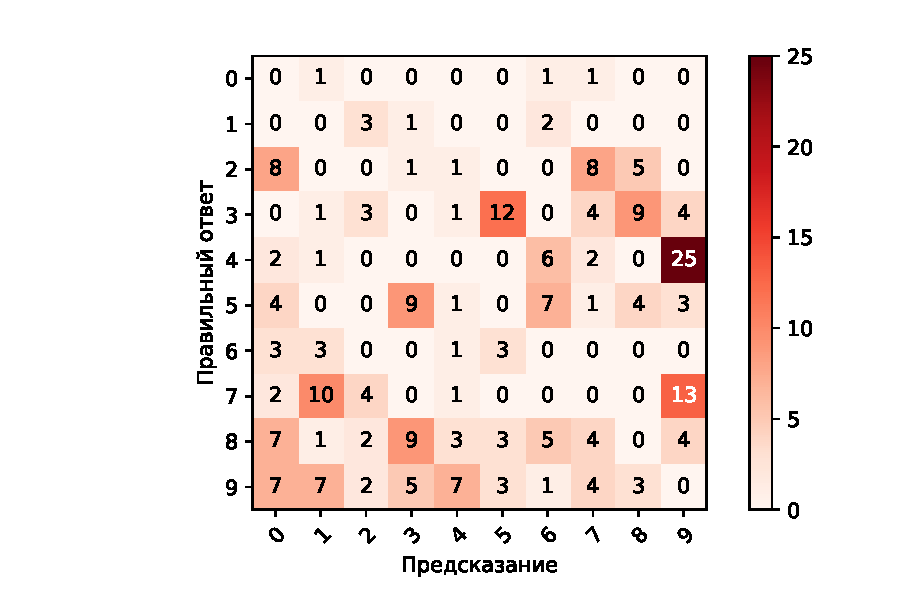
\includegraphics{../conf_matrix_experiment_4.pdf}

\begin{tabular}{c|cc}
    a & a & a
\end{tabular}




\end{document}